\documentclass[../main.tex]{subfiles}

% Importing images from another path
\graphicspath{{\subfix{../images/}}}

\begin{document}

The details of the implemented models, as well as the collection of the latencies data, are strictly connected to the architecture on which the benchmarks have been conducted. In particular, the \textit{EPYC} partition of the \textit{ORFEO} cluster has been used for the measurements. Nodes of this partition are equipped with two sockets with AMD EPYC 7H12 (Rome) cpus installed, for a total of $128$ cores per node~\cite{epyc}. Inside each of these cpus, cores are organized in $4$ NUMA regions. Each region contains then $2$ Core Complex Die (CCD), which in turn contain $2$ Core Complexes (CCX) with $4$ cores each that share the L3 cache~\cite{Velten2022}.\\
Hence, the \cc{osu\_bcast} and \cc{osu\_reduce} benchmarks have been used on $2$ EPYC nodes to collect the latencies of all the algorithms presented in sections~\ref{algorithms} for various numbers of processes in the range $[2,256]$ and for multiple message sizes from $1$ B up to $2^{20}$ B. Additionally, since the \cc{map-by} flag of the \textit{OpenMPI} library offers the interesting possibility of allocating MPI processes in this architecture according to different policies, these measurements have been conducted for the all three of the following mapping policies: 
% \begin{itemize}
%     \item \cc{map-by core}: processes are allocated to cores in a round-robin fashion;
%     \item \cc{map-by socket}: processes are allocated to sockets in a round-robin fashion;
%     \item \cc{map-by node}: processes are allocated to nodes in a round-robin fashion.
% \end{itemize}
\begin{itemize}[itemsep=0pt]
    \item \cc{map-by core}: processes are allocated to cores in a round-robin fashion;
    \item \cc{map-by socket}: processes are allocated to sockets in a round-robin fashion;
    \item \cc{map-by node}: processes are allocated to nodes in a round-robin fashion.
\end{itemize}
Concerning the point-to-point communications, a premise is needed. As introduced in section~\ref{algorithms}, the execution time of the different algorithms is also related to the specific communication channel $c$ used during the single point-to-point transmissions. This study tries to model the complex architecture of the EPYC node considering $4$ possible channels:
\begin{itemize}[itemsep=0pt]
    \item the \textbf{cache} channel ($0$), used by processes in the same CCX sharing the L3 cache;
    \item the \textbf{core} channel ($1$), used by processes allocated in the same socket;
    \item the \textbf{socket} channel ($2$), used by processes in the same node, but in different sockets;
    \item the \textbf{node} channel ($3$), used by processes allocated in different nodes.
\end{itemize}
The numbers in brackets hint to the fact that channels are ordered according to the increasing latency of the point-to-point communications as later explained in equation~\ref{eq:channels-order}, under the assumption that such order remains constant for all algorithms and message sizes.\\
This specific channel modelling therefore guided the measurements of the point-to-point latencies in the following way. For each of the $4$ channels, the \cc{osu\_latency} test has been run multiple times by allocating one process in a constant fixed position of one node while increasingly changing the core allocation of the other process until all the possible combinations had been tested. This allowed to map the point-to-point latencies of the different channels as represented in figure~\ref{fig:p2p-channels}.
Moreover, since these measurements have been repeated for different message sizes, the data collected for each channel have been linearly fitted as a function of the message size in order to model the single point-to-point communications of each channel using the Hockney model~\cite{Hockney}:
\begin{equation}\label{eq:hockney}
    \widehat{T}^{c}_{p2p}(m) = \alpha^{c} + \beta^{c} \cdot m
\end{equation}
where $\alpha^{c}$ and $\beta^{c}$ are respectively the latency and the inverse bandwidth of the channel $c$.\\
Finally, one last measurements has been conducted in order to obtain an estimate for the \textit{parallelization factor} $\gamma^{c}(P,m)$ previously introduced. Since for each channel the number of processes exclusively using that specific channel ranges from $2$ up to $P^{\max(c)}_{NBFT}$, the execution time $T^{c,m}_{NBFT}(P)$ of a NBFT that only uses one channel $c$ have been measured for all possible values of $P \in [2,P^{\max(c)}_{NBFT}]$ and all channels. This has been repeated for multiple message sizes $m$ and the measured values have then been fitted accoridng to the relation  
\begin{equation}\label{eq:nbft-fit}
    \widehat{T}_{NBFT}^{c,m}(P) = \alpha^{c,m} + \beta^{c,m} \cdot (P-1)
\end{equation}
where $\alpha^{c,m}$ is the latency of the NBFT and $\beta^{c,m}$ is the cost in the latency of a NBFT due to the addition of one process to the communication in the same channel $c$. According to equation~\ref{eq:nbft-approx}, these fits have then been used to experimentally obtain the discrete function:
\begin{equation}\label{eq:gamma-discrete}
    \widehat{\gamma}^{c}(P,m) = \frac{\widehat{T}_{NBFT}^{c,m}(P)}{\widehat{T}^{c}_{p2p}(m)} \quad \forall P \in [2,P^{\max(c)}_{NBFT}]\;,\;\forall m
\end{equation}
that serves as a platform-specific but algorithm-independent estimation of $\gamma^{c}(P,m)$.
\begin{figure}[h]
    \centering
    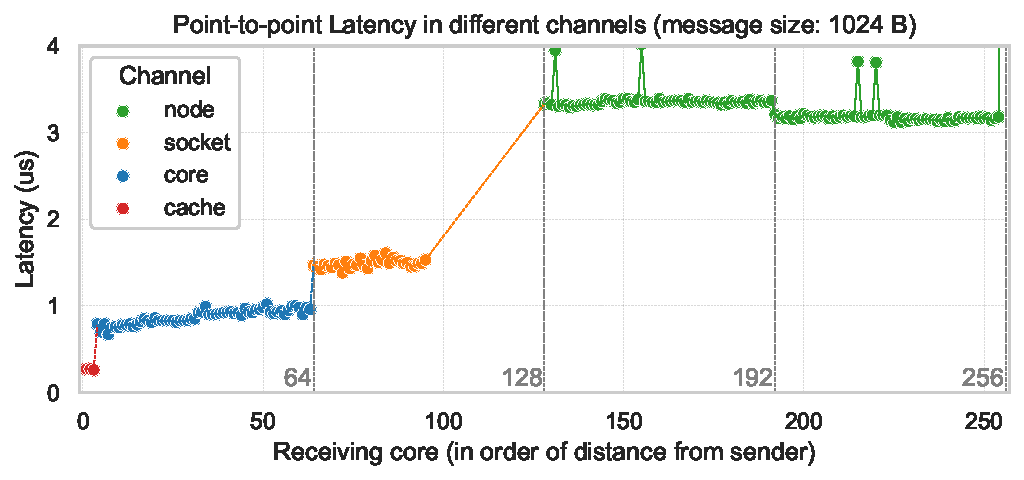
\includegraphics[width=\textwidth]{p2p-channels.pdf}
    \caption{Point-to-point latencies for all possible receiving cores in different channels of the $2$ EPYC nodes. Socket channel is missing values from $96$ to $127$ due to outliers.}
    \label{fig:p2p-channels}
\end{figure}

\end{document}